% !TeX spellcheck = eu_ES
\documentclass[eu]{ifirak}\usepackage[]{graphicx}\usepackage[]{color}
%% maxwidth is the original width if it is less than linewidth
%% otherwise use linewidth (to make sure the graphics do not exceed the margin)
\makeatletter
\def\maxwidth{ %
  \ifdim\Gin@nat@width>\linewidth
    \linewidth
  \else
    \Gin@nat@width
  \fi
}
\makeatother

\definecolor{fgcolor}{rgb}{0.345, 0.345, 0.345}
\newcommand{\hlnum}[1]{\textcolor[rgb]{0.686,0.059,0.569}{#1}}%
\newcommand{\hlstr}[1]{\textcolor[rgb]{0.192,0.494,0.8}{#1}}%
\newcommand{\hlcom}[1]{\textcolor[rgb]{0.678,0.584,0.686}{\textit{#1}}}%
\newcommand{\hlopt}[1]{\textcolor[rgb]{0,0,0}{#1}}%
\newcommand{\hlstd}[1]{\textcolor[rgb]{0.345,0.345,0.345}{#1}}%
\newcommand{\hlkwa}[1]{\textcolor[rgb]{0.161,0.373,0.58}{\textbf{#1}}}%
\newcommand{\hlkwb}[1]{\textcolor[rgb]{0.69,0.353,0.396}{#1}}%
\newcommand{\hlkwc}[1]{\textcolor[rgb]{0.333,0.667,0.333}{#1}}%
\newcommand{\hlkwd}[1]{\textcolor[rgb]{0.737,0.353,0.396}{\textbf{#1}}}%

\usepackage{framed}
\makeatletter
\newenvironment{kframe}{%
 \def\at@end@of@kframe{}%
 \ifinner\ifhmode%
  \def\at@end@of@kframe{\end{minipage}}%
  \begin{minipage}{\columnwidth}%
 \fi\fi%
 \def\FrameCommand##1{\hskip\@totalleftmargin \hskip-\fboxsep
 \colorbox{shadecolor}{##1}\hskip-\fboxsep
     % There is no \\@totalrightmargin, so:
     \hskip-\linewidth \hskip-\@totalleftmargin \hskip\columnwidth}%
 \MakeFramed {\advance\hsize-\width
   \@totalleftmargin\z@ \linewidth\hsize
   \@setminipage}}%
 {\par\unskip\endMakeFramed%
 \at@end@of@kframe}
\makeatother

\definecolor{shadecolor}{rgb}{.97, .97, .97}
\definecolor{messagecolor}{rgb}{0, 0, 0}
\definecolor{warningcolor}{rgb}{1, 0, 1}
\definecolor{errorcolor}{rgb}{1, 0, 0}
\newenvironment{knitrout}{}{} % an empty environment to be redefined in TeX

\usepackage{alltt}

\usepackage{amsmath,latexsym,amssymb,natbib}
\usepackage{listings}
\usepackage{ifcommands,subfigure}
\usepackage[T1]{fontenc}
\usepackage{tcolorbox}

\newcommand{\zkk}{\guillemotleft}
\newcommand{\skk}{\guillemotright}
\IfFileExists{upquote.sty}{\usepackage{upquote}}{}
\begin{document}
\ikasturtea{2013/2014}
\irakasgaia{Bilaketa Heuristikoak}
\title{BHLN: Soluzio bakarrean oinarritutako algoritmoak}
\date{}
\irakaslea{Borja Calvo, Usue Mori}
\author{Borja Calvo, Josu Ceberio, Usue Mori}


\tel{943 01 50 13}
\mail{borja.calvo@ehu.es}


\maketitle

\begin{abstract}
Kapitulu honetan soluzio bakarrean oinarritzen diren algoritmoak aztertuko ditugu. Algoritmo eraikitzaileak mota honetakoak izan arren, teknikoki ez dira bilaketa heuristikoak -- ez dago bilaketa prozesurik -- eta, hortaz, ez ditugu kapitulu honetan azalduko. Horren ordez, bilaketa lokalari erreparatuz, lehenengo atalean bere inguruan agertzen diren kontzeptuak azalduko ditugu. Bilaketa lokalaren arazorik handiena optimo lokaletan trabatuta geratzea denez, kapituluaren bigarren zatian arazo hau saihesteko zenbait estrategia aztertuko ditugu.
\end{abstract}

\section{Kontzeptu orokorrak}
Bilaketa lokalaren atzean dagoen intuizioa oso sinplea da: soluzio bat emanda, bere \zkk inguruan\skk\ dauden soluzioen artean soluzio hobeak bilatzea. Ideia hau bilaketa prozesu bihurtzeko, uneoro problemarako soluzio (bakar) bat mantenduko dugu eta, bilaketaren pausu bakoitzean, uneko soluzio horren ingurunean dagoen beste soluzio batekin ordezkatuko dugu. 

Ideia honetan hainbat algoritmo oinarritzen dira, bakoitzak bere berezitasunekin, noski. Diferentziak diferentzia, zenbait elementu komunak dira algoritmo guztietan; atal honetan kontzeptu hauek aztertzeari ekingo diogu.

\subsection{Soluzioen inguruneak}

Bilaketa lokalean dagoen kontzepturik nagusiena inguruarena da -- \textit{neighborhood} ingelesez -- eta, hortaz, problema bat ebazterakoan arreta handiz diseinatu beharreko osagaia da. Ingurune funtzioak edo operadoreak\footnote{Programazio testuinguruetan -- sasikodetan, adibidez -- \zkk operadore\skk\ terminoa erabiliko dugu soluzioak maneiatzeko erabiltzen diren funtzioetarako. Definizio matematikoetan, berriz, \zkk funtzio\skk\  terminoa erabiliko dugu, gehien bat.}, soluzio bakoitzeko, bilaketa espazioaren azpimultzo bat itzultzen du.

\begin{ifdefinition}
Izan bedi $\cal S$ bilaketa espazioa; $N:{\cal S} \rightarrow 2^{\cal S}$ funtzioari, $s\in {\cal S}$ soluzioa emanda bilaketa $N(s)\subset {\cal S}$ espazioaren azpimultzo itzultzen duenari, ingurune funtzioa deritzo
\end{ifdefinition}

Soluzio baten ingurunean dauden soluzioak antzerakoak izatea espero dugu; alabaina, ingurune operadoreek soluzioen kodeketarekin dihardute. Beraz, bilaketa lokal bat diseinatzean ondo aukeratu behar da kodeketa/ingurune bikotea, ingurunean dauden soluzioak antzerakoak izan daitezen. Ezaugarri honi lokaltasuna --\textit{locality} ingelesez-- esaten zaio, eta emaitza onak lortzeko funtsezkoa da.

\begin{tcolorbox}
\begin{ifexample}{\bf Lokaltasuna FSS probleman}
Datu meatzaritzan, gainbegiratutako datu base bat daukagunean, sailkatzaile funtzioak eraikitzea edo ikastea ataza oso ohikoa da. Funtzio hauek, beraien izenak adierazten duen moduan, datu berriak sailkatzeko erabiltzen dira. 

Oro har, datuetan dauden aldagaiek iragarpenak egiteko gaitasun ezberdinak dituzte; are gehiago, aldagai batzuk eragin negatiboa izan dezakete sailkatzailearen funtzionamenduan. Hori dela eta, aldagaien azpi-multzo bat aukeratzea oso pausu ohikoa da; prozesu hau, ingelesez {\em feature subset selection, FSS} deitzen dena, optimizazio problema bat da. FSS problemarako soluzioak bektore bitarren bidez kode daitezke, bit bakoitzak dagokion aldagaia azpi-multzoan dagoenetz adierazten duelarik. 

Bektore bitarrek zenbaki osoak moduan interpreta daitezke eta, hortaz, antzerako soluzioak zenbaki horiei balio txikiak gehituz/kenduz sor ditzakegu. Adibidez, $(01001)$ soluzioa badugu $9$ zenbakia moduan interpreta dezakegu eta, hortaz, antzerako soluzioak lor ditzakegu 1 gehituz -- $(01010)$, hau da, $10$ zenbakia -- edo kenduz -- $(01000)$, $8$ zenbakia --. Adibide honetan lortutako soluzioak nahiko antzerakoak dira; lehendabiziko kasuan azken aldagaia azken-aurrekoarekin ordezkatu dugu eta bigarren kasuan azken aldagaia kendu dugu. Edonola ere, beste kasu batzuetan lokaltasuna ez da mantentzen; $(1000000)$ soluzioari 1 kentzen badiogu, $(0111111)$ lortuko dugu, hau da, aukeratuta zegoen aldagai bakarra -- lehendabizikoa -- kendu eta beste gainontzeko guztiak sartu.

Lokaltasun falta dela eta, ingurune operadore ohikoena {\em flip} aldaketan oinarritzen dena da; inguruneko soluzioak sortzeko uneko soluzioaren posizio batean dagoen balioa aldatzen da, hau da, 0 bada 1ekin ordezkatzen da eta 1 bada, 0rekin. Operadore honekin FSS probleman beti bermatzen da lokaltasuna, ingurunean dauden edozein bi soluziok aldagai bakar bateko diferentzia izango baitute.
\end{ifexample}
\end{tcolorbox}

Soluzioak bektoreen bidez kodetzen direnean, inguruneak definitzeko \zkk distantzia\skk\ kontzeptua erabili ohi da, esplizituki zein inplizituki. Era honetan, bi soluzio bata bestearen ingurunean daudela esango dugu baldin eta beraien arteko distantzia finkaturiko kopurua baino txikiagoa bada. Bi soluzioen arteko distantzia $d(s,s^\prime)$ funtzioaz adierazten badugu, ingurunearen definizio orokorra hauxe izango da:

\begin{align}
N(s;k) = \{s^\prime\ |\ d(s,s^\prime)\leq k\}
\end{align}

Bektorearen motaren arabera distantzia ezberdinak erabil ditzakegu. Jarraian adibide hedatuenak ikusiko ditugu.

\noindent{\bf Bektore errealak} - Bektore errealekin dihardugunean euklidearra da gehien erabiltzen den distantzia

\begin{eqnarray*}
d_e(s,s^\prime) = \sqrt{\sum_{i=1}^n (s_i^\prime - s_i)^2}
\end{eqnarray*}


Ingurune tamainari erreparatuz, zenbaki errealak direnez infinitu soluzio izango ditugu edozein soluzioren ingurunean. Euklidearra distantziarik ezagunena izan arren, badira beste metrika batzuk ere -- Manhanttan- edo Chevyshev-distantziak, besteak beste --.

\noindent{\bf Bektore kategorikoak eta bitarrak} - Bektoreetan dauden aldagaiak kategorikoak direnean, bi bektoreen arteko distantzia neurtzeko metrikarik ezagunena Hamming-ek proposatutakoa da: $d_h(s,s^\prime) = \sum_{i=1}^n I(s_i\neq s_i^\prime)$ da, non $I$ funtzioak 1 balioa hartzen du bere argumentua egia denean eta 0 beste kasuan; hau da, Hamming-distantziak posizioz posizioko desberdintasunak neurtzen ditu. Hamming-distantzia inguruneak definitzeko erabiltzen denean ohikoena 1 distantziara dauden soluzioak erabiltzea da, hau da:

\begin{align}\label{eq:hamming1_neigh}
N_{h1}(s) = \{s^\prime\in {\cal S}\ |\ d_h(s,s^\prime) = 1\}
\end{align}

Algoritmoak diseinatzean oso garrantzitsua da ingurunearen tamaina aztertzea. Aurreko operadorea $n$ tamainako bektore bitar bati aplikatzen badiogu, $|N(s)| = n$ izango da, posizio bakoitza aldatzeko aukera bakarra baitaukagu. Bektore kategorikoetan, posizio bakoitzean $r_i$ balio hartzeko aukera dagoenean, ingurunearen tamaina $|N(s)| = \sum_{i=1}^n (r_i - 1)$ izango da.

Ingurune funtzio hau orokor daiteke edozein distantziarako -- distantzia maximoa bektorearen tamaina dela kontutan hartuz, betiere  --.:

\begin{align}
N_{hk}(s;k) = \{s^\prime\in {\cal S}\ |\ d_h(s,s^\prime) \leq k\}
\end{align}

\noindent{\bf Permutazioak} - Permutazioen arteko distantziak neurtzeko metrikak existitu arren, ingurune operadore klasikoak ez dituzte zuzenean erabiltzen. Horren ordez, permutazioetan definitutako eragiketak erabili ohi dira, trukaketa eta txertaketa batik bat. Trukaketan -- \textit{swap} ingelesez --, permutazioaren bi posizio hartzen dira eta beraien balioak trukatzen dira. Adibidez, $[21345]$ permutazioa badugu, 1. eta 3. posizioak trukatzen baditugu $[31245]$ permutazioa lortuko dugu. Formalki, trukaketa funtzioa defini dezakegu $t_r(s;i,j)$ non $s^\prime = t_r(s;i,j)$ bada $s^\prime(i)=s(j)$, $s^\prime(j)=s(i)$ eta $\forall k\neq i,j$ $s^\prime(k)=s(k)$ beteko den. Funtzio onetan oinarriturik, ondoko operadorea defini dezakegu:

\begin{align}
N_{2opt}(s) = \{t_r(s;i,j)|\ 1 \leq i,j\leq n, i > j\}
\end{align}

Operadore honi \textit{2-opt neighborhood} deritzo, bi posizio bakarrik trukatzen baitira. Era berean, operadorea hedatu ahal da trukaketa gehiago eginez. Hedatzeaz gain, operadorea murriztu ere egin ahal da, bakarrik elkarren ondoan dauden posizioak trukatuz.

Ingurunearen tamainari dagokionez, posizio jarraien trukaketak eginez $n$ ingurune soluzio izango ditugu; edozein bi posizio trukatzen baditugu, berriz, ingurunearen tamaina $n(n-1)$ izango da.

Txertaketa egitean elementu bat permutaziotik atera eta beste posizio batean sartzen dugu. Adibidez, $[54123]$ permutaziotik abiatuta, bigarren elementua laugarren posizioan txertatzen badugu, emaitza $[51243]$ izango da. Eragiketa $t_x(i,j)$ funtzioaren bidez adieraziko dugu -- $i$ elementua $j$ posizioan txertatu --, ingurunearen definizioa hauxe izango da:

\begin{align}
N_{in}(s) = \{t_x(s;i,j)|\ 1 \leq i,j\leq n, i \neq j\}
\end{align}

Trukaketan bakarrik bi posizio aldatzen dira; txertaketan, berriz, bi indizeen artean dauden posizio guztiak aldatzen dira. Hori dela eta, ingurune operadore bakoitzaren erabilgarritasuna problemaren araberakoa izango da. 

Bi inguru operadore hauetaz gain, literaturan beste zenbait topa daitezke, inbertsio eragiketan oinarritutakoak, adibidez.


\subsection{Optimo lokalak}

Bilaketa lokalean -- oinarrizko bertsioan, behintzat -- soluzio batetik bestera mugitzeko helburu funtzioa hobetu behar da eta, beraz, algoritmoa bukatzean uneko soluzioak ($s^*$) ondoko baldintza beteko du:

\begin{align*}
\forall s \in N(s^*)\ \ f(s^*)\leq f(s)
\end{align*}

Ekuazio hau optimo globalarenaren oso antzerakoa da; alabaina, optimo globalaren kasuan, bilaketa espazio osoan bete behar da eta hemen, berriz, bakarrik $s^*$ soluzioaren ingurunean daudenentzat. Soluzio guztietarako betetzen bada, $s^*$ \textit{optimo globala} dela esaten da; ildo berean, inguruko soluzioentzat bakarrik betetzen baldin bada, $s^*$ \textit{optimo lokala} dela esango dugu.

\begin{figure}[t]
\centering
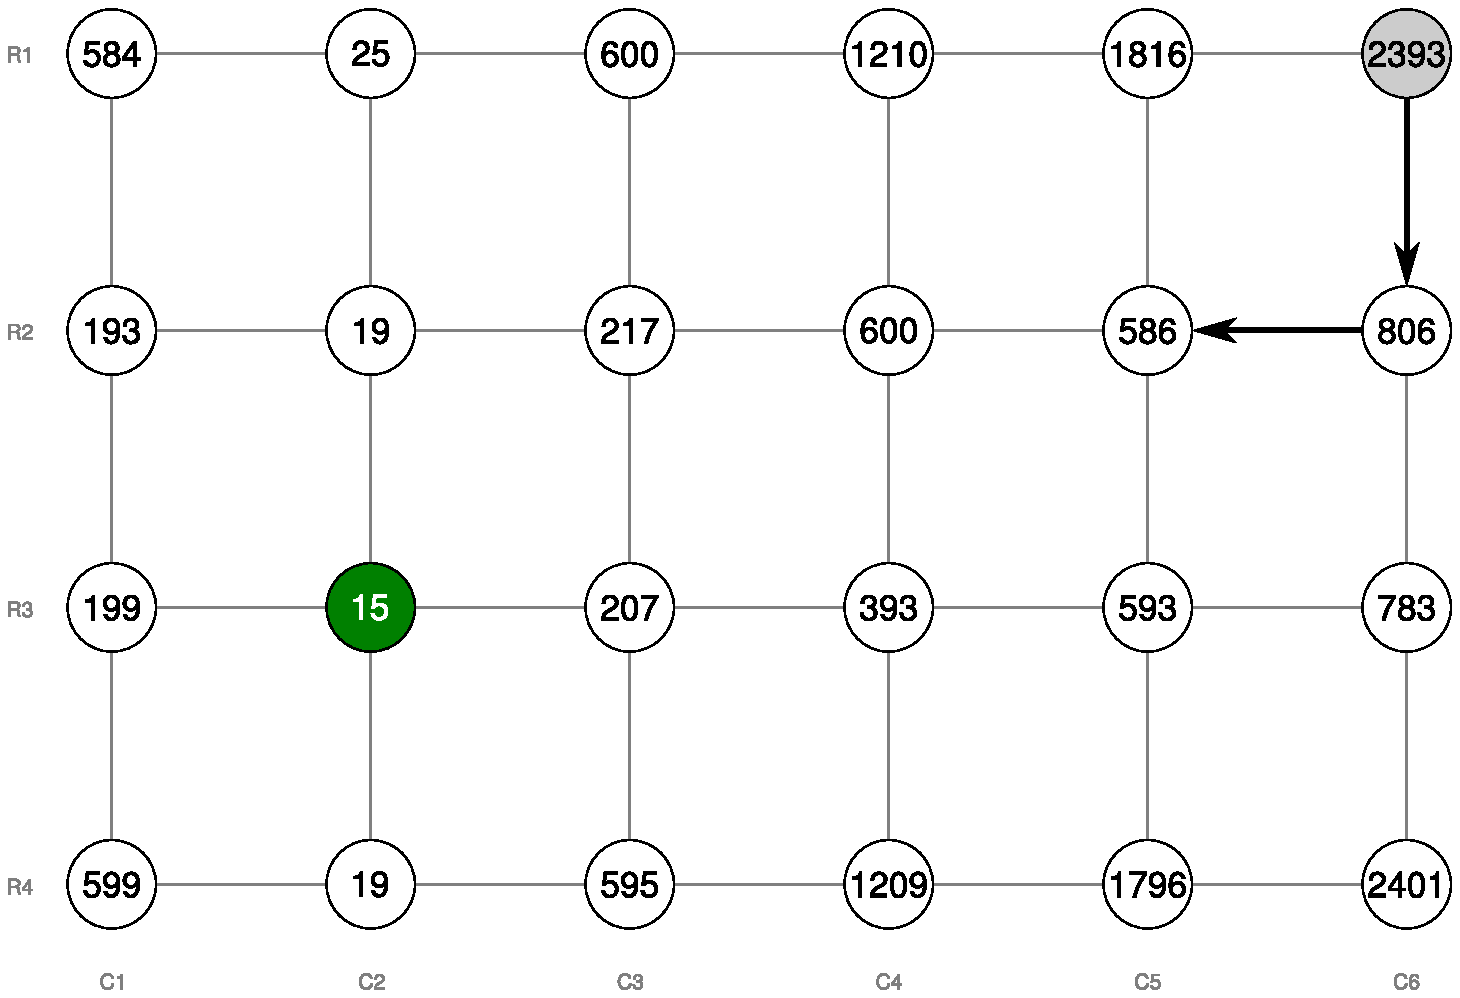
\includegraphics[width=0.66\linewidth]{./Irudiak/local_optimum}
\caption{Optimo lokalaren adibidea. Goiko eskumako soluziotik abiatzen bada bilaketa -- (R1,C6), grisean nabarmendua dagoen soluziotik, alegia --, pausu bakoitzean aukerarik onena aukeratuko bagenuke, geziek markatzen duten bidea jarraitu eta, bi pausutan, (R2,C5) soluzioan trabatuta geldituko ginateke. Soluzio hau optimo lokala da, bere inguruneko soluzio guztiak txarragoak baitira. Optimo lokalaren ebaluazioa 586 da, oso txarra optimo globalarekin alderatzen badugu.}
\label{fig:local_optimum}
\end{figure}

Ondorioz, bilaketa lokala optimo lokal batean amaitzen da beti. Hauxe da, hain zuzen, bilaketa lokalaren ezaugarririk -- eta, aldi berean, arazorik -- nagusiena. Aintzat hartzekoa da optimo lokalak, nahiz eta bere inguruneko soluziorik onenak izan, nahiko soluzio txarrak izan daitezkeela, \ref{fig:local_optimum} irudian erakusten den bezala. Irudi honetan kapituluan zehar erabiliko dugun grafiko mota bat ikus daiteke. Grafikoan fikziozko problema baterako soluzio guztiak jasotzen dira, bakoitza borobil baten bidez adierazita; borobilen barruan soluzio bakoitzaren helburu funtzioaren balioa idatzita dago. Ingurunearen funtzioa soluzioak lotzen dituzten marren bidez adieraziko da; bi soluzio lotuta badaude, bata bestearen ingurunean dago. 

\begin{tcolorbox}
\begin{ifexample}
\ref{fig:local_optimum} irudian agertzen diren geziek algoritmoak egiten duen bidea erakusten dute, (R1,C6) soluziotik abiatuta. Pausu bakoitzean inguruneko soluziorik onena aukeratzen badugu, algoritmoa bi pausutan trabatuta geldituko da (R2,C5) soluzioan; soluzio honen ebaluazioa 586 da eta, bere ingurunean dauden soluzioen ebaluazioak handiagoa direnez -- 1816, 806, 593 eta 600 --, ez dago helburu funtzioa hobetzen duen soluziorik. (R2,C5) optimo lokal bat da eta, optimo globalaren -- (R3,C2) -- ebaluazioa 15 dela kontutan hartuz, nahiko soluzio txarra gainera.
\end{ifexample}
\end{tcolorbox}

Optimo lokaletatik ateratzeko hainbat estrategia planteatu dira literaturan, bilaketa lokalaren puntu batean edo bestean aldaketak proposatuz. Hauxe izango da, hain juxtu, \ref{sec:BLHedapenak}. atalean aztergai izango duguna.

Ikusi dugunez, edozein soluziotik abiatuta, bilaketa lokala beti optimo lokal batean amaitzen da. Are gehiago, bi soluzio ezberdinetatik hasita, bilaketa lokala soluzio berdinean amaitu ahal da. Beste era batean esanda, optimo lokalek soluzioak \zkk erakartzen\skk\ dituzte, zulo beltzak balira bezala. Ideia hau \zkk erakarpen-arroa\skk\ -- \textit{basin of attraction}, ingelesez -- deritzon kontzeptuan formalizatzen da eta, gero ikusiko dugun moduan, oso garrantzitsua da problemen zailtasuna aztertzerakoan.

\begin{ifdefinition}{\bf erakarpen-arroa}
Izan bitez $N$ ingurune funtzioa, $f$ helburu funtzioa, $A(s;f,N): {\cal S}\rightarrow {\cal S}$ bilaketa lokala eta $s^*$ optimo lokala ($N$ ingurunerako eta $f$ funtziorako). $s^*$ optimo lokalaren erakarpen-arroa $\{s \in {\cal S} / A(s;N,f)=s^*\}$ soluzio multzoa da.
\end{ifdefinition} 

Erakarpen-arroa, definizioan ikus daitekeen legez, helburu funtzioaren, ingurunearen eta algoritmoaren araberakoa da. Ingurunearen eta helburu funtzioaren eragina begi bistakoa da. Algoritmoari dagokionez, ingurunea nola aztertzen den eta, bereziki, zein soluzio aukeratzen den ezartzen du; ondorioz, egiten dugun ibilbidean eragina handia izan dezake, \ref{fig:ls_selection_effect} irudiak ikus daitekeen bezala.

\begin{figure}[t]
\centering
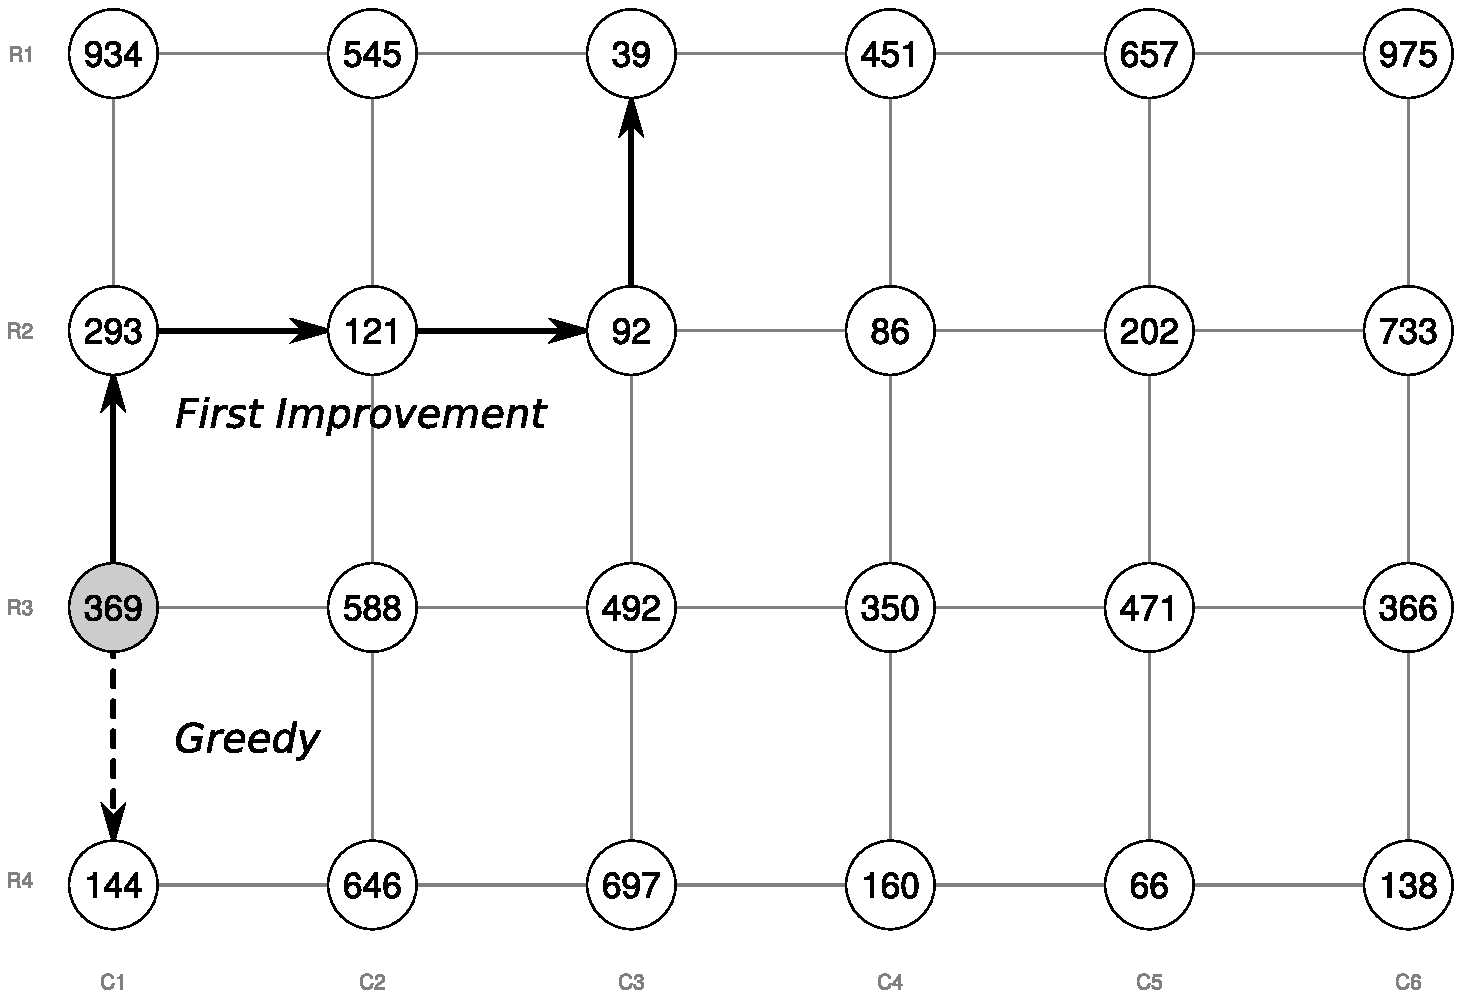
\includegraphics[width=0.66\linewidth]{./Irudiak/ls_selection_effect}
\caption{Inguruneko soluzioaren aukeraketaren efektua. Irudiak, soluzio berdinetik abiatuta -- (R3,C2), grisean nabarmendua -- bi estrategia ezberdin erabiliz egindako ibilbideak erakusten ditu. Lehenengo estrategia \textit{first improvement} motakoa da, hau da, helburu funtzioa hobetzen duen lehenengo soluzioa aukeratzen dugu -- inguruneko soluzioen ordena goikoa, eskumakoa, behekoa eta ezkerrekoa izanik --. Irizpide hau erabiliz egindako ibilbidea (R2,C1), (R2,C2), (R2,C3), (R1,C3) da, azken soluzio hau optimo lokala izanik. Bigarren estrategia gutiziatsua da -- \textit{greedy}-a, alegia --; hurrengo soluzioa ingurunean dagoen soluziorik onena izango da beti. Estrategia hau erabiliz pausu bakar batean (R4,C1) optimo lokalera ailegatzen gara}
\label{fig:ls_selection_effect}
\end{figure}



\subsection{Optimizazio problemen \zkk itxura\skk}

Bilaketa lokalean uneko soluziotik honen inguruan dagoen soluzio batera mugitzen gara beti, hau da, soluzio bakoitzetik zenbait soluzioetara mugi gaitezke. Hori dela eta, bilaketa espazioa grafo baten bidez adieraz daiteke non erpinak soluzioak dira eta ertzek mugimendu posibleak adierazte dituen; \ref{fig:local_optimum} irudiak horrelako grafo bat adierazten du.

Bilaketa espazioaren definizioari soluzioen ebaluazioa gehitzen badiogu optimizazio problemaren \zkk itxura\skk\ -- \textit{landscape}-a, ingelesez -- daukagu. Problemaren itxuraren eragina berebizikoa da algoritmoen performantzian eta, beraz, algoritmoak diseinatzerakoan kontuan hartu beharreko elementua da. Zentsu horretan, aintzat hartzekoa da problemaren arabera ez ezik, \textit{landscape}-a problema instantzia konkretuen arabera ere alda daitekeela.


\section{Bilaketa lokala}

\begin{ifalgorithm}[t]\label{alg:basicLS}
\begin{ifpseudo}{Oinarrizko bilaketa lokala}
\item \In\ $f$ helburu funtzioa, $s_0$ hasierako soluzioa, $N$ ingurune funtzioa
\item \Out\ $s^*$ soluzio optimoa
\item $s^*=s_0$
\item \Do
\item \T{$H=\{s^\prime \in N(s^*) | f(s^\prime)<f(s^*)\}$}
\item \T{\If $|H|>0$ }
\item \TT{Aukeratu $H$-n dagoen soluzio bat $s^\prime$ }
\item \TT{$s^* = s^\prime$}
\item \T{\EIf}
\item \While ($|H|>0$)
\end{ifpseudo}
\caption{Oinarrizko bilaketa lokalaren sasikodea. Uneko soluzioaren ingurunean helburu funtzioa hobetzen duen soluzio bat bilatzen dugu. Horrelakorik badago, uneko soluzioa ordezkatzen dugu; ez badago, bilaketa amaitzen da.}
\end{ifalgorithm}

\ref{alg:basicLS} algoritmoan oinarrizko bilaketa lokalaren sasikodea ikus daiteke. Zenbait gauza nabarmen daitezke algoritmo honetan. Lehenik eta behin, bilaketa soluzio batetik hasten da. Soluzio hau nola aukeratzen dugun erabakitzea garrantzitsua da, aurreko atalean ikusi dugun legez horren arabera optimo lokal batean edo bestean amituko baita bilaketa. Uneko soluzioaren ingurunean hainbat soluzio izango ditugu, beraz, zein aukeratuko dugu hurrengo uneko soluzioa izateko? Azkenik, sasikodean dagoen prozedura optimo lokal bat topatzen dugunean amaitzen da; dena dela, beste edozein algoritmotan bezala, denboran edota ebaluazio kopuruan oinarritutako gelditze irizpideak proposa ditzakegu.

Jarraian algoritmoaren bi aspektu garrantzitsu aztertuko ditugu: hasierako soluzioa eta inguruneko soluzioaren aukeraketa.

\subsection{Hasierako soluzioa}

Lehen aipatu bezala, bilaketa lokala soluzio batetik abiatuko da. Nondik hasi bilaketa oso garrantzitsua da, horren arabera optimo lokal batean edo bestean amaituko baitu bilaketa. Hau \ref{fig:local_optimum} irudian agerikoa da; (R1,C6) soluziotik hasten badugu bilaketa (C2,R5) soluzioan amaituko da. Gauza bera gertatzen da optimo lokaletik bertatik -- (C2,R5) --, goian dagoen soluziotik -- (C1,R5) -- edo bere eskuinean dagoen soluziotik -- (C2,R6) -- hasten bada prozesua. Beste edozein soluzio aukeratzen badugu, berriz, optimo globalera helduko gara. 

Bi dira bilaketa lokala hasieratzeko erabiltzen diren estrategiak:

\begin{itemize}
\item \textbf{Ausazko soluzioak erabiltzea} -  Ausaz aukeratzen da bilaketa espazioan dagoen soluzio bat. Metodo honen abantaila bere sinpletasuna da, ausazko soluzioak sortzea erraza izan ohi baita\footnote{Hau ez da beti egia; gure probleman murrizketa asko daudenean ausazko soluzioak sortzea oso zaila izan daiteke}. Estrategia honek alde txarrak ere baditu; alde batetik, hasierako soluzioa txarra bada, bilaketa prozesua luzea izan daiteke eta, bestetik, algoritmoa aplikatzen dugun bakoitzean emaitza, oro har, ezberdina izango da. Azken puntu hau optimo lokalen arazoa ekiditeko estrategiak diseinatzeko erabil daiteke, \ref{sec:multistart} atalean ikusiko dugun legez.
\item \textbf{Soluzio onak eraikitzea} - Lehenengo kapituluan ikusi genuen problemak ebazteko metodo heuristiko espezifikoak diseina daitezkeela. Oro har, metodo hauek pausuz pausu soluzio onak eraikitzen dituzte, urrats bakoitzean aukera guztietatik onena aukeratuz -- ingelesez metodo hauei \textit{constructive greedy} deritze, hau da algoritmo eraikitzaile gutiziatsuak edo jaleak --. Nahiko soluzio onak eman arren, hauek ez daukate zergatik optimoak\footnote{Ez optimo globalak eta ezta lokalak ere} izan behar eta, beraz, lortutako soluzioak bilaketa lokala hasieratzeko erabil daitezke. Estrategia hauek emaitza hobeak lortu ohi dituzte eta bilaketak iterazio gutxiago behar izaten dituzte; desabantaila nagusia, ordea, kostu konputazionala da.
\end{itemize}

\subsection{Inguruneko soluzioaren aukeraketa}

Behin inguruneko soluzioen multzoa definiturik, hurrengo pausua soluzioen aukeraketa irizpidea ezartzea da. Lehen aipatu bezala, bi dira, nagusiki, erabiltzen diren estrategiak: helburu funtzioa hobetzen duen lehenengo soluzioa aukeratzea edo helburua gehien hobetzen duen soluzioa bilatzea. Oro har, inguruneak txikiak direnean bigarren hurbilketa da interesgarriena; Hala eta guztiz ere, inguruneak handiak direnean, kostu konputazionala dela eta, bideraezina gerta daiteke.

Lehenengo hurbilketan inguruneko soluzioen \zkk ordenazioa\skk\ oso garrantzitsua da, uneko soluzioa hobetzen duen lehenengo soluziora mugituko baikara. 

\begin{tcolorbox}
\begin{ifexample}
Demagun problema baterako soluzioak bektore bitarren bidez kodetzen ditugula. Uneko soluzioa, zeinen helburu funtzioa $25$ den, $(0,1,1,0,1)$ da. Ingurunea definitzeko \eqref{eq:hamming1_neigh} ekuazioan dagoen funtzioa erabiltzen badugu, inguruneko soluzioak hauexek izango dira:
\begin{itemize}
\item $s_1=(1,1,1,0,1)$; $f(s_1)=30$
\item $s_2=(0,0,1,0,1)$; $f(s_2)=24$
\item $s_3=(0,1,0,0,1)$; $f(s_3)=5$
\item $s_4=(0,1,1,1,1)$; $f(s_4)=27$
\item $s_5=(0,1,1,0,0)$; $f(s_5)=29$
\end{itemize} 
Inguruneko soluzioak esploratzeko posizioak banan-banan aldatu behar ditugu. Lehenengo posiziotik abiatzen bagara, $s_2$ soluzioa izango da helburu funtzioa hobetzen duen lehenengoa, bere ebaluazioa $24$ baita. Azken posiziotik abiatzen bagara, berriz, $s_3$ soluzioarekin geldituko ginateke, ebaluazioa $5$ baita. Helburu funtzioa ez ezik, soluzioa ezberdina da eta, hortaz, hurrengo urratsean izango dugun ingurunea ezberdina izango da. Hori dela eta, inguruneko soluzioen azterketa alde batera edo bestera eginez azken soluzioa ezberdina izan daiteke.
\end{ifexample}
\end{tcolorbox}

Adibidean inguruneko soluzioak kodeketarekin zerikusia duen ordena erabiltzen da. Horren ordez, esplorazioa ausaz egin daiteke, helburua hobetzen duen soluzioetatik ausazko bat aukeratuz.

Inguruneak handiak direnean ordenak oso eragin handia izan dezake eta, hortaz, heuristikoak erabil daitezke esplorazioa egiteko. Adibide gisa, Fred Glover-ek TSP problemarako proposatutako \textit{ejection chains} \citep{pesch1997} aipa daitezke. 

Metodo heuristikoez gain, tamaina handiko inguruneak era eraginkorrean zehazki aztertzeko algoritmoak ere badaude; hauetako adibide bat \textit{dynasearch}\citep{congram2000} algoritmoa da.


\section{Bilaketa lokalaren hedapenak}\label{sec:BLHedapenak}

Aurreko atalean ikusi dugun legez, bilaketa lokala soluzioak areagotzeko prozedura egokia izan arren, arazo larri bat du; optimo lokaletan trabatuta gelditzen da. Arazo hau saihesteko -- soluzioen dibertsifikazioa suspertzeko, alegia -- bilaketa lokalak dituen lau aspektu nagusietan aldaketak sar ditzakegu: hasierako soluzioan, ingurunearen definizioan, inguruneko soluzioen aukeraketan eta helburu funtzioaren definizioan. Hurrengo ataletan elementu bakoitzean aldaketak sartzen dituzten algoritmo batzuk aurkeztuko ditugu.


\subsection{Hasieraketa anizkoitza}\label{sec:multistart}
Soluzio bakoitzetik abiatzen garenean optimo lokal batera heltzen gara; soluzio ezberdinetatik abitatzen bagara, optimo lokal ezberdinetara helduko gara. Ideia hau \ref{alg:randomMultistartLS} sasikodean inplementatuta dagoena da. Algoritmoan agertzen diren \textit{random\_solution} eta \textit{local\_search} funtzioetan dago prozeduraren mamia. Batak espazioaren esplorazioa egiten du eta besteak, bere izenak adierazten duen bezala, soluzioen areagotzeaz arduratzen da.


\begin{ifalgorithm}[t]
\begin{ifpseudo}{Hasiera-anizkoitza bilaketa lokal orokorra}
\item \In\ $f$ helburu funtzioa
\item \In\ \textit{random\_solution}, \textit{stop\_criterion} eta \textit{local\_search} funtzioak
\item \Out\ $s^*$ soluzioa optimoa
\item $s$=\textit{random\_solution}
\item \While{!\textit{stop\_criterion}}
\item \T{$s^\prime$ = \textit{random\_solution}}
\item \T{$s^{\prime\prime}$ = \textit{local\_search}($s^\prime$)}
\item \T{\If({$f(s^{\prime\prime})<f(s)$}) $s=s^{\prime\prime}$}
\item \Done
\end{ifpseudo}
\caption{Hasieraketa anizkoitza erabiltzen duen bilaketa lokalaren hedapenaren sasikode orokorra}\label{alg:randomMultistartLS}
\end{ifalgorithm}


Ausazko soluzioak sortzeko hainbat aukera ditugu. Lehendabizikoa uniformeki ausaz sortzea da, hots, pasu bakoitzean probabilitate berdinarekin espazioaren edozein soluzioa aukeratuko dugu, bilaketa lokala hasieratzeko. 

Uniformeki ausazko soluzioetatik abiatzea problema gehienetan aukera erraza da; alabaina, ez da oso estrategia adimentsua. Gainera, murrizketa askoko problemetan ausazko soluzio bideragarriak sortzea zaila izan daiteke. Ausazko soluzio \zkk onak\skk\ eraikitzeko prozedura bat izanez gero bi arazo hauek saihes ditzakegu. Hain juxtu, hauxe da GRASP algoritmoan egiten dena; hasierako soluzio multzo sortzeko heuristiko gutiziatsu bat erabili, gero \textit{random\_solution} funtzioak multzo horretatik soluzioak ausaz ateratzeko. Ausazko soluzioak sortzeko beste aukera bat aurreko pausuan lortutako optimo lokaletik abiatzea da, ILS algoritmoan egiten den legez.


\subsubsection{Bilaketa Lokala Iteratua (ILS)}

Bilaketa lokala berrabiarazteko ausazko soluzioak erabili beharrean, ILS -- \textit{Iterated Local Search}, ingelesez -- algoritmoan uneko optimo lokala hartuko dugu oinarritzat. Ideia oso sinplea da; optimo lokal batean trabaturik gelditzen garenean, soluzioa \zkk perturbatu\skk\ eta bilaketarekin jarraituko dugu. Optimo lokal berri batera heltzean, soluzio hau onartuko dugunetz erabaki behar dugu. \ref{alg:ILS} algoritmoan ILS-aren sasikode orokorra ikus daiteke.

\begin{ifalgorithm}[t]
\begin{ifpseudo}{Bilaketa Lokala Iteratua (ILS)}
\item \In\ $f$ helburu funtzioa
\item \In\ \textit{accept}, \textit{perturb}, \textit{stop\_criterion} eta \textit{local\_search} funtzioak
\item \In\ $s_0$ hasierako soluzioa
\item \Out\ $s^*$ soluzioa
\item $s = $ \textit{local\_search}($s_0$)
\item $s^* = s$
\item \While{!\textit{stop\_criterion}}
\item \T{$s^\prime$ = \textit{perturb}($s$)}
\item \T{$s^{\prime\prime}$ = \textit{local\_search}($s^\prime$)}
\item \T{\If (\textit{accept}($s^{\prime\prime}$)) $s=s^{\prime\prime}$}
\item \T{\If{($f(s^{\prime\prime})<f(s^*)$)} $s^*=s^{\prime\prime}$}
\item \Done
\end{ifpseudo}
\caption{Bilaketa Lokala Iteratuaren (ILS) sasikodea}\label{alg:ILS}
\end{ifalgorithm}


Bi prozedura dira algoritmo honetan definitu behar ditugunak:

\begin{itemize}
\item \textbf{Perturbazioa} - Bilaketa lokalean soluziotik soluziora mugitzeko aldaketa txikiak egiten dira. Optimo lokaletatik ateratzeko, beraz, egin behar diren aldaketak handiagoak izan beharko dira. Hau \ref{fig:ILS} irudiak ikus daiteke. Perturbazioa txikiegia izango bazen -- (R1,C5) soluziora mugitzea, adibidez --, berriro optimo lokal berdinean amaituko zen bilaketa. Perturbazioa nahiko handia bada, uneko optimo lokalaren erakarpen-arrotik aterako gara eta, definizioz, beste optimo lokal batean trabaturik geldituko gara. Kontutan hartzekoa da perturbazio prozedurak itzulitako soluzioa erabat ausazkoa bada --hau da, perturbazioa oso handia bada --, ILS algoritmoa ausazko hasieraketa anizkoitz algoritmoa bilakatuko dela. Perturbazioaren tamaina egokitzea ez da erraza, problemaren \textit{landscape}-arekin zerikusia baitu eta, lehen ikusi dugun moduan, hau instantziatik instantziara alda daiteke.

Perturbazioa definitzean inguruneko soluzioak definitzeko mugimendu mota berberak edo beste batzuk erabil daitezke. Esate baterako, permutazioetan oinarritzen den problema batean \textit{2-opt} ingurune operadorea erabiltzen badugu, \textit{k-opt} operadorea erabil daiteke soluzioak perturbatzeko. Perturbazioa trukaketan oinarritu beharrean, txertaketa ere erabil dezakegu, $k$ elementu hartu eta ausazko posizioetan sartuz. 

Perturbazioaren tamaina aurretik finkatu eta bilaketaren zehar aldatu barik mantendu ahal da. Estrategia estatiko honen ordez, estrategia dinamikoak erabil daitezke, non tamaina bilaketaren zehar aldatzen den.

Soluzioak perturbatzeko prozedura aurreratuetan bilaketaren \zkk historia\skk\ erabil daiteke, soluzioaren zein osagai perturbatu eta zein ez erabakitzeko. Estrategia hauek \zkk memoria\skk\ kontzeptua erabiltzen dute; erabiltzen diren mekanismoak -- memoria motak -- tabu bilaketan soluzioak areagotzeko eta dibertsifikatzeko erabiltzen direnen antzerakoak dira.

\item \textbf{Optimo lokalak onartzeko irizpideak} - Uneko optimo lokala perturbatu ondoren bilaketa lokala aplikatzen da, optimo (berri) bat sortuz. Hurrengo iterazioan lortutako optimo berria edo optimo zaharra perturbatuko dugun erabaki behar da. Bi hurbilketa estremo plantea daitezke: beti optimo berria onartu edo unekoa baino hobea denean bakarrik onartu. Lehendabiziko estrategiak dibertsifikazioa suspertzen du; bigarrenak, berriz, areagotzeko egokia da. Ohikoena tarteko zerbait erabiltzea da, optimo zaharraren eta berriaren arteko ebaluazioaren diferentzia kontutan hartuz. Esate baterako, optimoak era probabilistikoan onar daitezke, Boltzmann-en distribuzioa erabiliz, gero \textit{simmulated annealing} algoritmoan ikusiko dugun bezala. 
\end{itemize}

\begin{figure}[t]
\centering
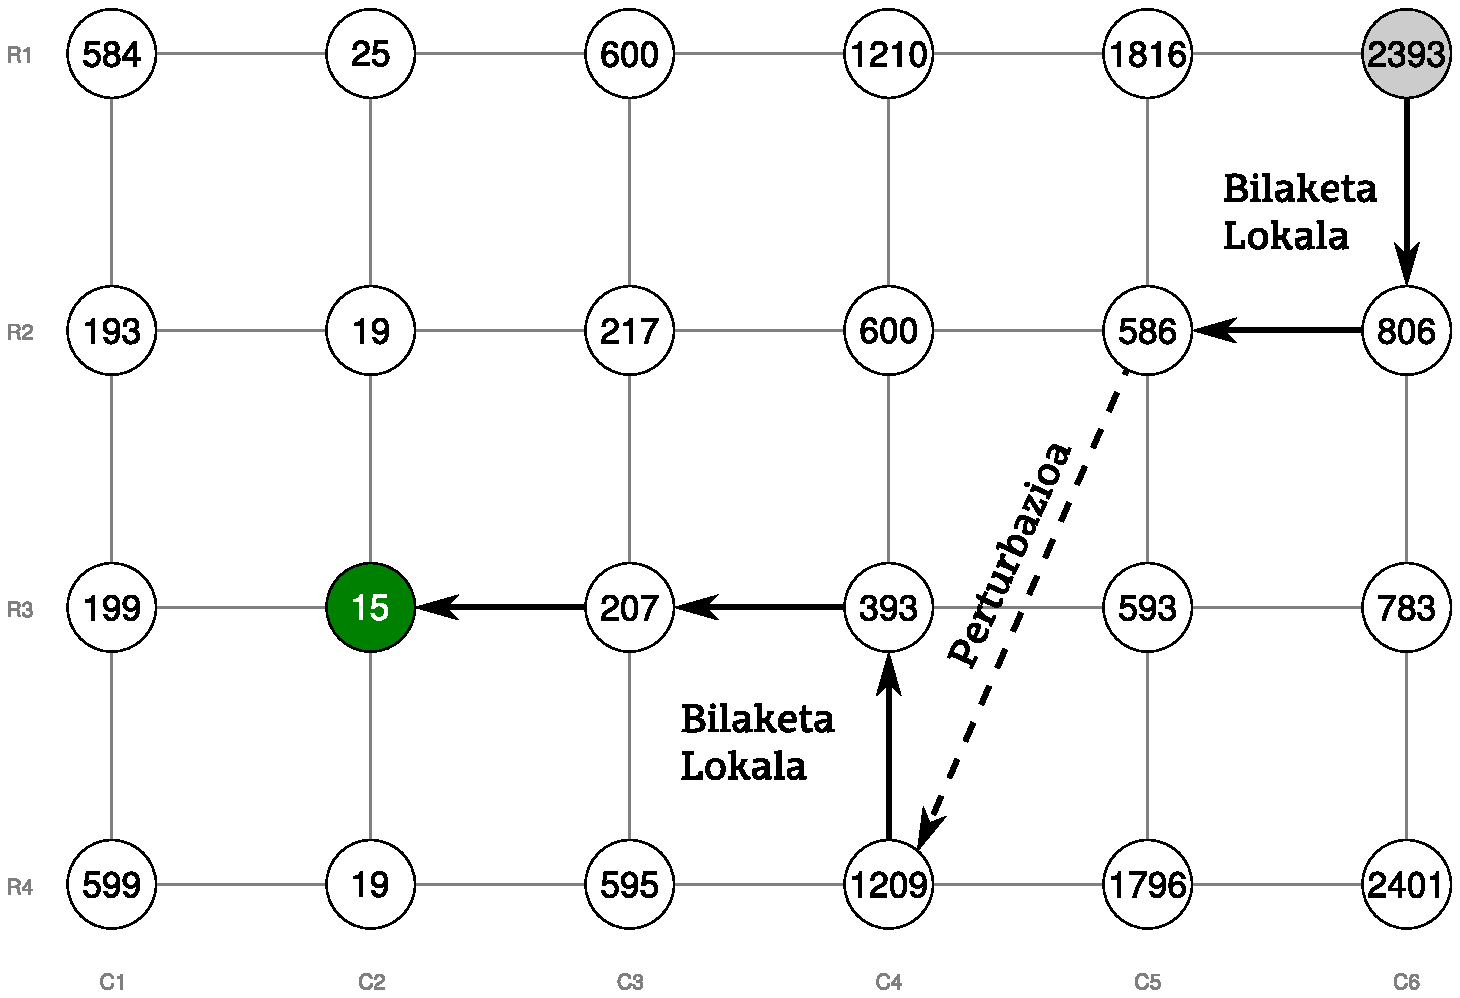
\includegraphics[width=0.66\linewidth]{./Irudiak/ILS}
\caption{ILS algoritmoaren funtzionamendua. Goiko eskumako soluziotik abiatzen bada bilaketa -- (R1,C6), grisean nabarmendua dagoen soluziotik, alegia --, (R2,C5) optimo lokalean trabatuta geldituko ginateke. Egoera desblokeatzeko soluzioa \zkk perturbatzen\skk\ dugu, (R3,C4) soluziora eramanez; hortik abiatuta bilaketa lokala aplikatzen dugu, kasu honetan optimo globalera heldu arte}
\label{fig:ILS}
\end{figure}


\subsubsection{GRASP algoritmoa}

Optimizazio problemak ebazteko ohiko da metodo eraikitzaileak erabiltzea. Aurreko kapituluan ikusi genuen bezala, algoritmo hauek soluzio pausuz pausu eraikitzen dute, urrats bakoitzean aukera guztietatik onena hautatuz. Era honetan, soluzio onak sortzen dira baina, berdinketak egon ezean, instantzia bakoitzeko soluzio bakarra lortzen dugu.

Metodo hauen bidez lortutako soluzioak onak izan arren ez daukate zergatik optimoak izan, ez globalki eta ezta lokalki ere. Hori dela eta, behin soluzioa sortuta, bilaketa lokal bat erabil daiteke soluzioa areagotzeko.

Ideia hau apur bat landuz, metodo eraikitzaileak soluzio bakarra sortu beharrean soluzio multzo bat sortzeko egoki ditzakegu. Gero, \ref{alg:randomMultistartLS} algoritmoan dagoen \textit{random\_solution} metodoak multzo horretatik ausazko soluzioak aterako ditu, bilaketa lokala hasieratzeko. Ideia hau GRASP \textit{Greedy Randomized Adaptative Search Procedure} algoritmoaren atzean dagoena da \cite{feo1989}.

Ausazko soluzio onak eraikitzeko, pausu bakoitzean aukerarik onena aukeratu beharrean \zkk hautagai zerrenda\skk\ izango dugu -- \textit{candidate list}, ingelesez --; algoritmoak zerrenda horretan dauden osagaiak ausaz aukeratuko ditu hasierako soluzioak eraikitzeko.

\begin{tcolorbox}
\begin{ifexample}
Demagun motxilaren problema ebatzi nahi dugula. Oso sinplea den algoritmo eraikitzaile bat hauxe da: kalkulatu, motxilan sartzek ditugun elementu bakoitzeko balioa/pisua ratioa eta gero, pausu bakoitzean, motxilan sartu ahal diren elementuetatik (pisu-muga gaindiarazi ez dutenak) ratiorik handiena duena aukeratu. 

Algoritmo hau GRASP algoritmoa inplementatzeko egoki daiteke. Algoritmoaren iterazio bakoitzean soluzio bat eraikiko dugu, pausu bakoitzean ratiorik handiena duen elementua aukeratu beharrean ratio handienak duten $\%\alpha$ soluzioen artetik bat ausaz aukeratuz. Behin soluzioa eraikita, bilaketa lokala aplikatuko dugu lortutako soluzioa areagotzeko. 
\end{ifexample}
\end{tcolorbox}


\subsection{Inguruneko soluzioen hautaketa}

Definizioz, optimo lokalak diren soluzioen inguruko soluzio guztiak bera baino txarragoak dira; hortaz, ez dugu soluzio hoberik aukeratzerik eta, ondorioz, bilaketa lokala trabatuta gelditzen da. Bilaketa prozesuari amaiera ez emateko, soluzio hoberik egon ezean, helburu funtzioa hobetzen ez duten soluzioak onar ditzakegu. Estrategia honi esker, txarragoak diren soluzio batzuetatik pasatuz gero bilaketa espazioaren eskualde hobeetara ailega gintezke.

Soluzio \zkk txarrak\skk\ aukeratzeko bi estrategia daude. Lehendabizikoan helburua hobetzen ez duen soluzio bat aukeratzean sortutako \zkk galera\skk\ kontutan hartzen da, era probabilistikoan zein deterministan. Algoritmorik ezagunena \textit{suberaketa estokastikoa} --\textit{simulated snnealing}~\cite{kirkpatrick1983,cerny1985} ingelesez-- izenekoa da, zeinek probabilitate-banaketa parametriko bat erabiltzen duen aukeraketa egiteko. Algoritmo honetan inspiratutako beste hainbat algoritmoak proposatu dira, \textit{demon algoritm}~\cite{pepper2000} eta \textit{threshold accepting}~\cite{dueck1990,moscato1990} algoritmoak, besteak beste.

Estrategia honen beste interpretazioa Gloverrek 1986an proposaturiko \textit{tabu bilaketa}~\cite{glover1986} --\textit{tabu search} ingelesez-- algoritmoarena da. Kasu honetan helburu funtzioa hobetzen ez duten soluzioak aukeratzen dira baldin eta soilik baldin ingurune osoan helburua hobetzen duen soluziorik ez badago. Estrategia honen arriskua dagoeneko bisitatu ditugun soluzioak bisitatzea den legez, \zkk memoria\skk erabili beharra dago zikloak saihesteko.

\subsubsection{Suberaketa Simulatua}

Tresnak edo piezak sortzeko prozesatzen direnean, metalek hainbat propietate gal dezakete, euren kristal-egituran eragindako aldaketak direla eta. Propietate horiek berreskuratzeko metalurgian \zkk suberaketa\skk\ prozesua erabiltzen da; metal pieza oso tenperatura handira berotzen da, gero astiro hozten uzteko. Tenperatura igotzean metalaren atomoen energia handitzen da eta, hortaz, beraien artean sortzen diren indar molekularrak apurtzeko gai dira; mugitzeko askatasun handiagoa dute, alegia. 

Metala oso azkar hozten bada --tenplatzean egiten den bezala, adibidez-- molekulak zeuden tokian \zkk izoztuta\skk\ gelditzen dira. Honek metala gogortzen du, baina hauskorragoa bihurtzen du, aldi berean. Suberatzean, berriz, metala poliki-poliki hozten da eta, ondorioz, molekulak astiro galtzen dute beraien energia --hots, abiadura--. Hozketa-abiadura motelari esker molekulak euren kristal-egiturako \zkk kokapen optimora\skk\ joaten dira, hau da, energia minimoko kristal-egitura sortzen da.

1983an Kirkpatrick-ek~\cite{kirkpatrick1983} eta bi urte geroago Cerny-k~\cite{cerny1985}, suberaketaren prozesuan inspiratuta, optimizazio algoritmoak proposatu zituzten; Kirpatrick-ek bere algoritmoari \textit{simmulated annealing}, suberaketa simulatua, izena eman zion eta hauxe da gaur egun hedatuen dagoena.

Algoritmoaren funtzionamendua sinplea da oso. Soluzio batetik ($s$) txarragoa den beste soluzio batera ($s^\prime$) mugitzeko, \zkk energia\skk\ behar dugu; behar den energia bi soluzioen ebaluazioen arteko diferentzia izango da, hau da, $\Delta E = f(s^\prime) - f(s)$. 

Energia-muga hau gainditzeko sistemak energia behar du; sistemaren energia \zkk tenperatura\skk ren bidez neurtuko dugu. Beste era batean esanda, uneoro sistemak $T$ tenperatura izango du eta, zenbat eta tenperatura altuago, orduan eta errazago izango da energia-mugak gainditzea.

Zehazki, soluzio batetik bestera mugitzeko gainditu behar den energia-muga gainditzen denetz erabakitzeko Boltzmann probabilitate-banaketa erabiltzen da:

\begin{align*}
P(\Delta E, T) = e^{-\frac{\Delta E}{T}}
\end{align*}

Ikus daitekeenez, distribuzio esponentzial honetan muga gainditzeko probabilitatea --hots, helburua hobetzen ez duen soluzioa onartzekoarena-- tenperaturarekiko proportzionala da; energia diferentziarekiko, ostera, alderantzizko proportzionala da.

Aintzat hartzekoa da $\Delta E<0$ denean funtzioaren balioa 1 baino handiagoa dela. Izanez, ekuazioa bakarrik energia diferentzia positiboa denean erabiltzen da, negatiboa bada $s^\prime$ soluzioa hobea baita eta, ondorioz, beti onartzen da.

\begin{ifalgorithm}[t]
\begin{ifpseudo}{Suberaketa Simulatua - Simulated Annealing}
\item \In\ \textit{random\_neighbor} operadorea
\item \In\ \textit{update\_temperature}, \textit{equilibrium}, \textit{stop\_condition} operadoreak
\item \Out\ $s^*$ topatutako soluziorik onena
\item $s^*=s$
\item $T=T_0$
\item \While {!\textit{stop\_condition}}
\item \T{\While{!\textit{equilibrium}}}
\item \TT{$s^\prime$ = \textit{random\_neighbor($s$)}}
\item \TT{$\Delta E = f(s^\prime)-f(s)$}
\item \TT{\If{$\Delta E < 0$}}
\item \TTT{$s=s^\prime$}
\item \TTT{\If{($f(s)<f(s^*)$)} $s^*=s$}
\item \TT{\EIf}
\item \TT{\Else}
\item \TTT{$e^{-\frac{\Delta E}{T}}$ probabilitatearekin $s=s^\prime$}
\item \T{\Done}
\item \T{T=\textit{update\_temperature(T)}}
\item \Done
\end{ifpseudo}
\caption{Suberaketa Simulatuaren sasikodea}\label{alg:SA}
\end{ifalgorithm}

Suberaketaren gakoa hozte-abiadura da eta, era berean, suberaketa simulatuaren zati garrantzitsuena izango da. Izan ere, hasieran $T$ balio handiak erabiliko ditugu, ia edozein soluzio onartzeko, eta gero, astiro, $T$ txikiagotuko dugu, optimo lokal batean trabatuta gelditu arte. \ref{alg:SA} algoritmoan suberaketa simulatuaren sasikodea ikus daiteke.

\begin{figure}[t]
\centering
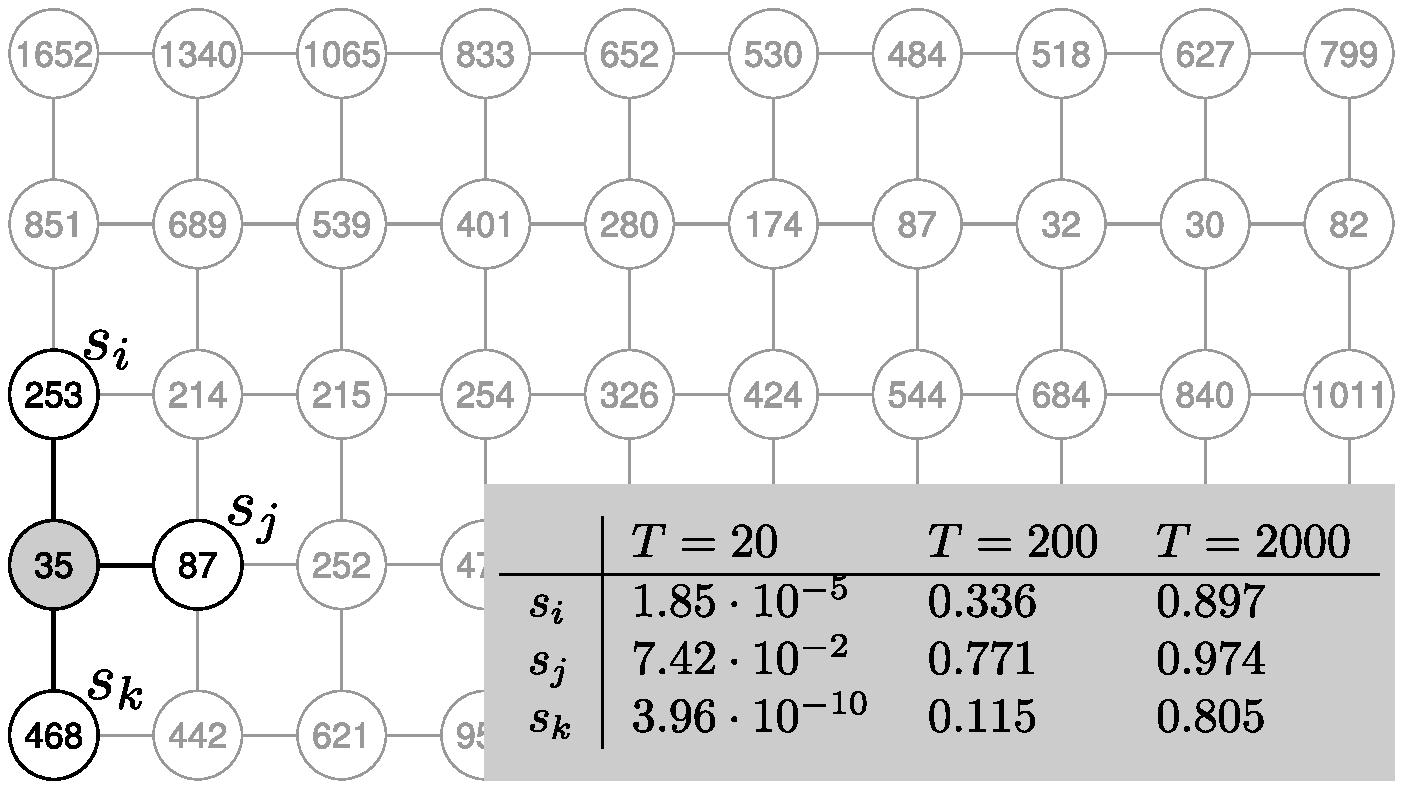
\includegraphics[width=0.66\linewidth]{./Irudiak/example_boltzman_dist}
\caption{Soluzioak onartzeko probabilitateen adibideak. Uneko soluzioa grisez nabarmendua dagoena izanik hiru soluzio ditugu ingurunean, $s_i,s_j$ eta $s_k$. Taulak soluzio bakoitza onartzeko probabilitateak jasotzen ditu, hiru tenperatura ezberdinekin. Ikus daitekeenez, tenperatura baxua denean edozein soluzioa aukeratzeko probabilitatea oso baxua da; tenperatura oso altua denean, berriz, edozein soluzioa hartuta litekeena onartzea da.}
\label{fig:example_boltzman_dist}
\end{figure}


Suberaketa simulatuaren motako algoritmoak diseinatzean lau aspektu hartu behar ditugu kontutan:
\begin{itemize}
\item \textbf{Hasierako tenperatura} - Altuegia bada, hasierako iterazioetan \textit{random walk}, hau da, ausazko ibilbide bat jarraituko dugu; baxuegia bada, berriz, bilaketa oinarrizko bilaketa lokala bihurtuko da. \ref{fig:example_boltzman_dist} irudian adibide bat ikus daiteke. $T=20$ denean, nahiz eta helburu funtzioen diferentzia txikia izan, soluzioa onartzeko probabilitatea txikia da; $T=2000$ denean ebaluazioen arteko diferentzia handia izan arren, litekeena soluzioak onartzea da. $T=200$ denean, berriz, optimo lokaletik atera gaitezke, probabilitate handiarekin, $s_j$ aukeratuz; aldi berean, tarteko tenperatura honekin oso soluzio txarrak onartzea zaila izango da. 

Tenperatura hasieratzeko bi estrategia ditugu. Lehendabizikoa tenperatura oso altua erabiltzea da; dibertsifikazio ikuspegitik interesgarria izan arren, estrategia hau konputazionalki garestia izan daiteke. Beste estrategian bilaketa espazioaren itxura aztertuko dugu, ingurunean dauden soluzioen arteko diferentziak nolakoak diren jakiteko. Gero, informazio hau onarpen ratio edo probabilitate ezagun bat lortzeko behar dugun tenperatura finkatzeko erabil daiteke~\cite{huang1986,aarts1987}.


\begin{tcolorbox}
\begin{ifexample}
Demagun 10 tamainako TSP-aren instantzia bat ebatzi nahi dugula. Kostu matrizean dagoen baliorik handiena -- hau da, bi hirien arteko distantziarik handiena -- 7.28 da. Problemarako soluzio guztietan 10 hiri izango ditugu eta, hortaz, soluzio guztien ebaluazioa matrizean dauden 10 elementuen batura izango da. Hori dela eta, $f_g=7.28 \cdot 10=78.2$ problema honetarako ebaluazio funtzioaren goi-muga bat da\footnote{Kontutan hartuz aipatutako baturan matrizeko elementuak ezin direla errepikatu, goi-muga birfindu daiteke 10 elementurik handienak batuz}. Era berean, matrizeko distantziarik txikiena 2.5 izanik, behe-muga kalkula ditzakegu: $f_b = 2.5\cdot 10$. Beraz, edozein soluzio aukeratzeko hasierako probabilitatea finkatzen badugu -- 0.75, adibidez --, bi muga hauek hasierako tenperatura kalkulatzeko erabil dezakegu, edozein bi soluzioen arteko ebaluazioaren diferentzia $f_g-f_b$ baino txikiagoa izango dela baitakigu:

\begin{align*}
P=0.75= e^{-\frac{f_g-f_b}{T_0}} = e^{-\frac{78.2-25}{T_0}}\\
T_0 = -\frac{78.2-25}{\ln(0.75)} = 184.93
\end{align*}

Beraz, hasierako tenperatura 185 balioan finkatzen badugu, badakigu hasierako iterazioetan edozein soluzio aukeratzeko probabilitatea \%75 edo handiagoa izango dela.
\end{ifexample}
\end{tcolorbox}

\item \textbf{Oreka lortzeko iterazio kopurua} - Tenperatura balio bakoitzeko zenbait iterazio egin behar dira -- hau da, zenbait inguruneko soluzio aztertu behar da -- \zkk oreka\skk\ lortu arte. Behin oreka lorturik, tenperatura eguneratu behar da, berriro oreka bilatzeko. Lehenengo pausua, beraz, oreka lortzeko behar dugun iterazio kopurua ezartzea da. Ohikoena inguruneko tamainaren araberako iterazio kopurua finkatzea da. Beste era batean esanda, aurretik $\rho$ ratioa finkatuko dugu; gero, tenperatura bakoitzeko $\rho|N(s)|$ soluzio ebaluatuko ditugu, non $|N(s)|$ uneko soluzioaren ingurunearen tamaina den. 

Estrategia honetan iterazio kopurua finkatuta dago, baina badaude beste estrategiak non kopurua tenperatura bakoitzeko aldakorra den. Adibide gisa, tenperatura soluzio berri bat onartzen dugun bakoitzean alda dezakegu; batzuetan ebaluatzen dugun lehendabiziko soluzioa onartuko dugu eta, bestetan, hainbat soluzio probatu beharko ditugu, bat onartu arte. Kasu honetan, beraz, iterazio kopurua aldakorra da. Ingurunean soluzio on asko badaude, iterazio gutxi beharko ditugu; kontrako kasuan, inguruneko soluzio gehienak txarrak badira, iterazio gehiago beharko ditugu uneko soluzio aldatzeko.

\item \textbf{Tenperatura jaitsieraren abiadura} - Hau da, ziurrenik, algoritmoaren osagairik nagusiena. Hainbat formula erabil daitezke tenperatura eguneratzeko. Hona hemen batzuk:
  \begin{itemize}
  \item \textit{Lineala}: $T_i=T_0 - i\beta$, non $T_i$ $i$ iterazioko tenperatura den. Eguneraketa honetan tenperatura beti positiboa izan behar dela kontrolatu behar dugu, ekuazioak tenperatura negatiboak itzuli baitaitezke.
  \item \textit{Geometrikoa}: $T_i = \alpha T_{i-1}$. $\alpha \in (0,1)$ abiadura kontrolatzen duen parametroa da eta, ohikoena, 0.5 eta 0.99 tartean egotea da.
  \item \textit{Logaritmikoa}: $T_i=\frac{T_0}{log(i)}$. Abiadura hau oso motela da baina, nahiz eta praktikan oso erabilgarria ez izan, algoritmoaren konbergentzia demostratuta dago ekuazio hau erabiltzen denean.
\end{itemize}
Funtzio guzti hauek monotonoak dira, hau da, iterazio bakoitzean tenperatura beti jaisten da. Edonola ere, problema batzuetan funtzio ez-monotonoek hobeto funtziona dezakete\footnote{Tenperatura igotzen denean dibertsifikazioan gailentzen da; tenperatura jaistean, berriz, areagotze prozesua indartzen da. Hau kontutan hartuz, funtzio ez-monotonoak dibertsifikazio/areagotze prozesuen arteko oreka kontrolatzeko erabil daitezke}.

\item \textbf{Algoritmoa gelditzeko irizpidea} - Aurreko puntuan ikusi dugu legez, iterazioak aurrera egin ahala tenperatura zero baliora hurbiltzen da baina, kasu gehienetan, ez da inoiz heltzen. Honek esan nahi du beti optimo lokaletatik ateratzeko aukera izango dugula, probabilitatea oso txikiarekin bada ere. Hori dela eta, algoritmoa gelditzeko baldintzaren bat beharko dugu. Irizpide hedatuena tenperatura minimo bat finkatzea da; bestela, denbora edota ebaluazio kopuru maximoak ere finka ditzakegu.
\end{itemize}

Ikusitako algoritmoetan soluzioen onarpena probabilistikoa da; alabaina, suberaketa simulatuaren kontzeptua era deterministan ere inplementa daiteke. Honen adibidea da Deabru Algoritmoa~\cite{pepper2000} -- \textit{Deamon Algorithm}, ingelesez --. Hasiera batean Creutz-ek algoritmoa simulazio molekularrak egiteko proposatu zuen, baina optimizazio problemak ebazteko ere egoki daiteke. Algoritmoan soluzioak onartuko direnetz erabakitzeko tenperatura erabili beharrean \zkk deabru\skk\ bat erabiltzen da; deabru honek uneoro $E_D$ energia du. Soluzio bakoitza aztertzerakoan, subaeraketa simulatuan legez, $\Delta E$ kalkulatzen da eta, une horretan $\Delta E>E_D$ bada, soluzioa onartzen da -- suberaketa simulatuan bezala, $\Delta E<0$ denean soluzioa onartzen da --. Algoritmoaren gakoa deabruaren energia eguneratzean datza; soluzio bat onartzen den bakoitzean deabruaren energia $E_D + \Delta E$ izatera pasatzen da, hau da, \zkk sistemaren\skk\ energia aldaketa deabruak jasotzen du. Onartutako soluzioa hobea denean, deabruak energia irabazten du eta, txarragoa denean, berriz, energia galtzen du -- energia nahiko baldin badu, betiere --. Algoritmo honen abantaila sinpletasuna da, Boltzmann distribuzioa ebaluatzeko beharrik ez baitugu.

\subsubsection{Tabu bilaketa}

Tabu bilaketa -- \textit{tabu search}, inglesez -- izango da, ziurrenik , bilaketa lokalaren aldaera hedatuena. Duen eraginkortasuna eta sinpletasuna dela eta, optimizazio konbinatorioan asko erabiltzen den eta, zenbait problematan, emaitzarik onenak ematen dituen metaheuristikoa da.

1977an lehenengo aldiz proposatuta, tabu bilaketak, optimo lokaletan trabaturik ez geratzeko, bilaketa soluzio txarragoetara bideratzea baimentzen du. Neurri honek prozesua amaigabeko ziklo batean sartzeko arriskua sortzen du, egindako bidea berregiteko aukera baitago. Arazo hori saihesteko, tabu bilaketak, bisitatutako soluzioen historikoa gordetzen du.

\begin{ifalgorithm}[t]
\begin{ifpseudo}{Tabu Bilaketa}
\item \In\ \textit{intensify} eta \textit{diversify} operadoreak
\item \In\ \textit{intensify\_condition}, \textit{diversify\_condition} eta \textit{stop\_condition} baldintzak
\item \In\ $\cal N$ ingurune operadorea eta $s_0$ hasierako soluzioa
\item \Out\ $s^*$ topatutako soluziorik onena
\item $s^*=s_0$
\item $s = s_0$
\item Hasieratu tabu zerrenda, epe erdiko memoria eta epe luzeko memoria
\item \While {!\textit{stop\_condition}}
\item \T{Topatu ${\cal N}(s)$-n dagoen soluzio onargarririk onena $s^\prime$}
\item \T{$s = s^\prime$}
\item \T{Eguneratu tabu lista}
\item \T{\If{\textit{intensify\_condition}}}
\item \TT{\textit{intensify}}
\item \T{\EIf}
\item \T{\If{\textit{diversify\_condition}}}
\item \TT{\textit{diversify}}
\item \T{\EIf}
\item \Done
\end{ifpseudo}
\caption{Tabu bilaketaren sasikodea}\label{alg:tabu}
\end{ifalgorithm}


Oinarrizko tabu bilaketa, bilaketa lokal gutiziatsuan oinarritzen da, non \zkk tabu zerrenda\skk\ deitzen den bisitatutako soluzio multzo bat gordeko den uneoro. Urrats bakoitzean tabu ez diren -- bideragarriak diren, alegia -- inguruneko soluzioetatik onena aukeratuko dugu, helburu funtzioa hobetzen duen ala ez kontutan hartu barik. Tabu ez diren soluzioak bakarrik hartzen ditugunez aintzat, ez da ziklorik sortuko.

Bisitatutako soluzio guztiak gordetzen dituen zerrenda mantentzea ez da bideragarria; hori dela eta, tabu zerrendan azkenengoz bisitatutako soluzioak bakarrik gordeko ditugu. Algoritmoaren iterazio bakoitzean, aukeratutako soluzioa tabu zerrendara gehituko da, eta zerrendatik soluzio bat aterako da -- tabu zerrendak FIFO pilak dira, hau da, sartzen lehendabizikoa den elementua ateratzeko ere lehendabizikoa izango da--. Azken soluzioak bakarrik gordetzen direnez tabu zerrendari epe laburreko memoria esaten zaio.

Tabu zerrendan soluzioak gordetzen baditugu, eta zerrendaren tamaina $k$ bada $k$ tamainako zikloak ekiditeko gai izango gara. Edonola ere, eraginkortasuna dela eta, soluzio osoak maneiatzeak kostu handia lekarke. Hori dela eta, aukera egokiagoak ere aurki ditzakegu literaturan, atributuak gordetzea, besteak beste. Atributuak soluzioen zatiak, mugimenduak, edo soluzioen arteko desberdintasunak izan ohi dira. Soluzioen elementu hauek ebazten ari garen problemaren menpekoak dira eta, hortaz, aukera ugari proposatu daitezke, kasu bakoitzeko tabu lista eredu desberdin bat inplementatuz. Ikus dezagun adibide bat.

\begin{tcolorbox}
\begin{ifexample}
Demagun permutazioetan oinarritutako problema batean tabu bilaketa bat inplementatu nahi dugula. Bilaketa lokalak {\em 2-opt} ingurunea erabiltzen badu, soluzio batetik bestera mugitzeko $i$ eta $j$ posizioak trukatuko ditugu. Era honetan, tabu zerrendan bi posizio hauek gorde ditzakegu, alderantzizko trukaketa tabu bihurtuz. Esate baterako, uneko soluzioa $[13245]$ bada eta $[31245]$ soluziora mugitzen bagara, hurrengo urratsetan lehenengo eta bigarren posizioak trukatzea debekatuko dugu. Problemaren arabera, beste irizpide batzuk erabil genitzake. Adibide gisa, adibidean lehenengo posizioan $1$a eta bigarrenean $3$a egotea tabu egin genezake.
\end{ifexample}
\end{tcolorbox}

Soluzioen atributuak erabiltzen ditugunean memoria gutxiago behar dugu eta, hortaz, tabu zerrenda handiagoak erabil ditzakegu; edonola ere, aintzat hartzekoa da estrategia honekin tabu zerrenda baino txikiagoak diren zikloak ager daitezkeela. Horrez gain, diseinatutako atributuak oso zehatzak izan behar dira, bisitatu gabeko soluzio onak ezabatu ez ditzagun. Ildo honetan \textit{aspiration criteria} deritzen irizpideak erabili ohi dira bilaketa prozesuan soluzioak onartzeko, tabu izan arren. Esate baterako, uneko soluziotik, tabu den mugimendu bat erabiliz orain arte topatutako soluziorik onena baino hobea den soluzio bat lortzen badugu, soluzio horretara pasatuko gara.

Tabu zerrendaren tamainak, tabu bilaketaren portaera definitzen du; txikia baldin bada, espazioko eremu txikietan zentratuko da; handia bada, berriz, algoritmoak eremu zabalagoetara bultzatuko du bilaketa, soluzio asko tabu izango baitira. Ohikoena, lista tamaina aldakor bat erabiltzea izaten da, algoritmoaren portaera kasu bakoitzeko beharretara egokitzeko.

Tabu zerrendaz gain, bestelako aukera konplexuagoak, ere proposatu dira. Epe motzeko memoria erabiltzeaz gain, bilaketa prozesuan jasotako informazioa ere oso baliotsua izan daiteke algoritmoa gidatzeko. Informazio hau epe erdiko edota epe luzeko memorian gorde daiteke. Lehendabiziko kasuan soluzio onenen informazioa bakarrik gordeko dugu, bilaketa areagotzeko asmoarekin. Bigarren kasuan, berriz, bilaketa osoan soluzioen osagaien frekuentziak gordeko ditugu; frekuentzia hauek bisitatu ez ditugun eremuei antzemateko erabil daitezke -- hau da, bilaketa dibertsifikatzeko --.


\begin{tcolorbox}
\begin{ifexample}
TSP-rako soluzioak eraikitzeko hiri bakoitzetik zein hirira mugituko garen erabaki behar dugu. Algoritmo eraikitzaile tipikoan erabaki hori kostu matrizea begiratuz hartzen da, uneko hiritik bisitatu gabeko gertuen dagoen hira aukeratuz. Era berean, epe erdiko eta epe luzeko memoriak matrize karratu batean inplementa ditzakegu. Matrize hauetan, bisitatutako zenbat soluzioetan $i$ hiritik $j$ hirira joaten garen gordeko dugu. Epe erdiko memorian azken $k$ soluzio onenen informazioa bakarrik gordeko dugu, areagotze prozesuan gehien erabili direnak finkatzeko eta bilaketa falta diren loturetan zentratzeko. Epe luzeko memorian, berriz, bisitatu ditugun soluzio guztien informazioa gordeko dugu. Era honetan, bilaketa esploratu gabeko eremuetara eraman nahi badugu, gutxien erabilitako loturak erabiliz soluzioak sor ditzakegu, bilaketa prozesua bertatik abiatzeko.
\end{ifexample}
\end{tcolorbox}

\subsection{Bilaketa espazioaren itxura aldaketa}

Soluzio bakarrean oinarritzen diren algoritmoekin amaitzeko bilaketa espazioaren \textit{landscape}-a eraldatzen dituzten algoritmoak aztertuko ditugu. Zehazki, bi algoritmo ikusiko ditugu. Lehenengoak, VNS-ak, ingurune definizio ezberdinak erabiltzen ditu optimo lokaletatik ateratzeko. Bigarrenak, berriz, helburu funtzio berriak sortzen ditu optimo lokalen kopurua murriztekotan.

\subsubsection{Variable Neighborhood Search algoritmoa}

Bilaketa lokalean optimo lokal batean trabaturik gelditzen gara, definizioz bere ingurunean helburu funtzioa hobetzen duen soluziorik ez dagoelako baina, zer gertatuko litzateke ingurune definizioa aldatuko bagenuke?. Adibide gisa, demagun optimizazio problema bat dugula non soluzioak permutazioen bidez kodetzen ditugun. Bilaketa lokala aplikatzeko \textit{2-opt} operadorea erabiliko dugu -- hau da, \textit{swap} eragiketan oinarritutako ingurunea --. Izan bedi $[1432]$ soluzioa, ingurune eta problema honetarako optimo lokala dena, hau da, edozein bi posizio trukatuz lortutako soluzioak txarragoak dira. Txertaketan oinarritzen den ingurunea erabiliz \textit{2-opt} ingurunean ez dauden soluzioak lor ditzakegu -- lehenengo elementua azken elementuaren ostean txertatuz lortzen den $[4321]$ soluzioa, esate baterako --. Beraz, gerta daiteke \textit{2-opt} ingururako optimo lokala den gure soluzioa txertaketa erabiltzen duen ingurunerako optimoa ez izatea.

Ideia hau \textit{Variable Neighborhood Descent} (VND) algoritmoan erabiltzen da bilaketa lokala optimo lokaletan trabaturik gera ez dadin. \ref{alg:VND} algoritmoan VND-aren sasikodea ikus daiteke. 

\begin{ifalgorithm}[t]
\begin{ifpseudo}{VND algoritmoaren sasikodea}
\item \In\ $\mathbf{\cal N} = \{{\cal N}_1,\ldots,{\cal N}_k\}$ ingurune funtzioak
\item \In\ $s$ hasierako soluzioa
\item  $i=1$
\item  $s^* = s$
\item \While {$i\leq k$} \Do
\item \T{Bilatu $s^\prime$, ${\cal N}_i(s^*)$ inguruneko soluziorik onena}
\item \T{\If{$f(s^\prime<f(s^*)$}}
\item \TT{$s^*=s^\prime$}
\item \TT{$i=1$}
\item \T{\Else}
\item \TT{$i=i+1$}
\item \T{\EIf}
\item \Done
\end{ifpseudo}
\caption{VND algoritmoaren sasikodea}\label{alg:VND}
\end{ifalgorithm}

Algoritmoan ikusten den bezala, VND-an ingurune funtzio bakarra izan beharrean multzo bat daukagu. Lehenengo funtzioarekin hasita, iterazio bakoitzean uneko soluzioaren inguruneko soluziorik onena bilatzen dugu. Inguruneko soluzio guztiak txarragoak badira -- soluzioa uneko ingurunerako optimo lokala bada, alegia -- hurrengo ingurune funtziora pasatzen gara; ingurune funtzio gehiagorik egon ezean bilaketa amaitzen da. Iterazio batean inguruneko soluzio berri batera pasatzen garen bakoitzean, berriro hasierako ingurune definiziora bueltatzen gara.

Bilaketa amaitzeko baldintza kontutan hartuz, algoritmo honek itzultzen duen soluzioa \textit{ingurune definizio guztietarako optimo lokala} izango da.

\textit{Variable Neighborhood Search} algoritmoa VND-aren hedapen bat da, non iterazio bakoitzean, uneko ingurune definizioa erabiliz bilaketa lokala amaiera arte eramaten den. Hau da, helburu funtzioa hobetzen duen soluzio bat topatu arren uneko ingurune definizioa mantentzen dugu optimo lokal batera heldu arte. Behin optimo lokal batean, hurrengo ingurune definiziora mugitzen gara, VND-an legez, lortutako soluzioa ingurune guztietarako optimo lokala izan arte. \ref{alg:VNS} algoritmoak VNS-aren sasikodea erakusten du.

\begin{ifalgorithm} [t]
\begin{ifpseudo}{Oinarrizko VNS algoritmoaren sasikodea}
\item \In\ \textit{local\_search} bilaketa algoritmoa
\item \In\ $\mathbf{\cal N} = \{{\cal N}_1,\ldots,{\cal N}_k\}$ ingurune funtzioak
\item \In\ $s$ hasierako soluzioa
\item  $i=1$
\item  $s^* = s$
\item \While {$i\leq k$} \Do
\item \T{Aukeratu ausaz soluzio bat $s^\prime\in {\cal N}_i(s^*)$}
\item \T{$s^{\prime\prime} = $\textit{local\_search}($s^*$,${\cal N}_i$)}
\item \T{\If{$f(s^{\prime\prime}<f(s^*)$}}
\item \TT{$s^*=s^{\prime\prime}$}
\item \TT{$i=1$}
\item \T{\Else}
\item \TT{$i=i+1$}
\item \T{\EIf}
\item \Done
\end{ifpseudo}
\caption{VNS algoritmoaren sasikodea}\label{alg:VNS}
\end{ifalgorithm}


\subsection{\textit{Smoothing} algoritmoak}

Optimizatu behar dugun funtzioak optimo lokal asko dituenean, bilaketa lokalak ez dira oso metodo egokiak, globala ez den optimo batean trabaturik gelditzeko probabilitatea oso altua delako. Leuntze-metodoetan -- \textit{smoothing methods}, ingelesez -- iterazio bakoitzean jatorrizko helburu funtzioa eraldatu -- leundu -- egiten da, optimo lokal kopurua gutxitzeko asmoz; helburu funtzio berria erabiliz bilaketa lokala aplikatzen da. Behin bilaketa trabaturik -- optimo lokal batean --, helburu funtzioa berriro aldatzen da, aurreko iterazioan baino gutxiago leunduz. Helburu funtzio berri honekin eta aurreko iterazioan lortutako optimoarekin bilaketa lokala aplikatzen da, optimo berri bat lortuz. 

Iterazioz iterazioa leuntze-maila geroz eta txikiago eginez, azkenengo iterazioan problemaren jatorrizko helburu funtzioa erabiliko dugu, problemarako soluzioa topatzeko. 


\begin{figure}[t]
\centering
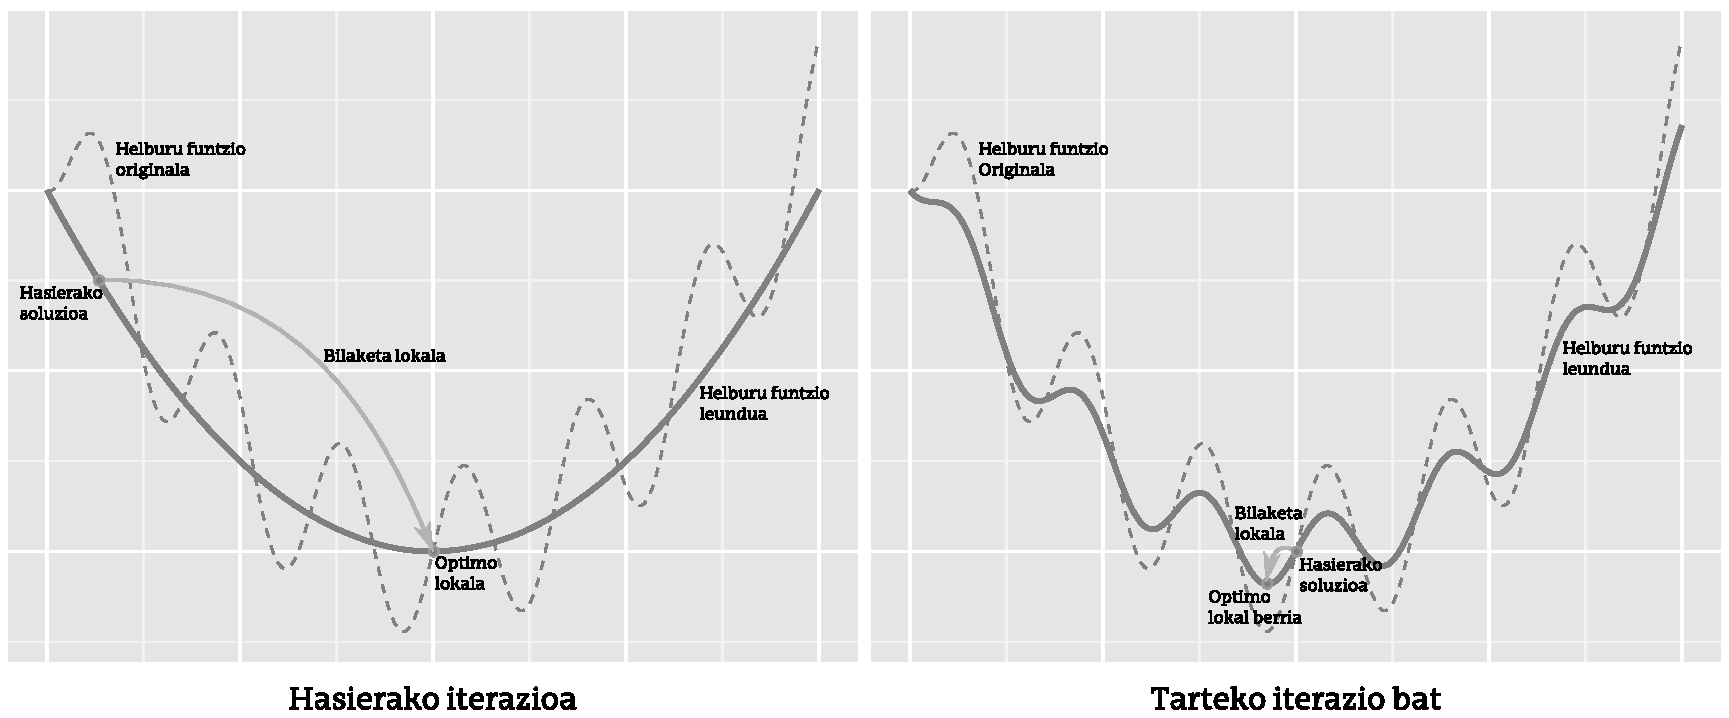
\includegraphics[width=0.75\linewidth]{./Irudiak/smoothing}
\caption{\textit{Smoothing} algoritmoaren funtzionamendua. Iterazio bakoitzean hasierako helburu funtzioa maila bateraino leuntzen da eta bilaketa lokala aplikatzen da.}
\label{fig:smoothing}
\end{figure}

Helburu funtzioa nola leundu problemaren araberakoa da. Edonola ere, kasu guztietan algoritmo inplementatu ahal izateko leuntze-parametro bat beharko dugu. Parametro hau handia denean, helburu funtzioa asko leunduko dugu; parametroa 1 denean, berriz, helburu funtzioa ez da bat ere aldatuko. Hau aintzat hartuz, \ref{alg:smooth} algoritmoan metodoaren sasikodea definituta dago. Ikus dezagun adibide bat.

\begin{ifalgorithm}[t]
\begin{ifpseudo}{\textit{Smoothing} metodoen sasikodea}
\item \In\ \textit{smoothing ($f$,$\alpha$)} helburu funtzioa eraldatzeko funtzioa
\item \In\ \textit{local\_search($s$,$f$)} bilaketa lokala
\item \In\ \textit{update($\alpha$)} faktorea eguneratzeko funtzioa
\item \In\ $s$ hasierako soluzioa; $\alpha_0$ hasierako faktorea; $f$ helburu funtzioa
\item  $s^* = s$; $\alpha=\alpha_0$
\item \While {$\alpha > 1$} \Do
\item \T{$f^\prime = $\textit{smoothing}($f$;$\alpha$)}
\item \T{$s^* = $\textit{local\_search}($s^*$,$f^\prime$)}
\item \T{$\alpha = $\textit{update}($\alpha$)}
\item \Done
\end{ifpseudo}
\caption{\textit{Smoothing} algoritmoaren sasikodea}\label{alg:smooth}
\end{ifalgorithm}


\begin{tcolorbox}
\begin{ifexample}

TSP-an helburu funtzioa kalkulatzeko distantzia matrizea erabiltzen dugu. Matrize horretan edozein bi hirien arteko distantzia jasota dugu. Helburu funtzioa leuntzeko matrizea eralda daiteke, distantzia guztiak batez-besteko distantziara gerturatuz, adibidez. Demagun ondoko matrizea definitzen dugula:

\begin{align}
\renewcommand*{\arraystretch}{1.5}
d_{ij}(\alpha) = \left\{
\begin{array}{ll}
\bar{d} + (d_{ij} - \bar{d})^\alpha &\ \ \mbox{baldin eta } d_{ij}\geq \bar{d}\\
\bar{d} - (\bar{d} - d_{ij})^\alpha &\ \ \mbox{baldin eta } d_{ij} < \bar{d}
\end{array}\right.
\end{align}

\noindent non $\bar{d}$ distantzien batez-bestekoa eta $d_{ij}$ jatorrizko matrizearen elementuak diren. Distantzia matrizea normalizaturik badago -- distantzia guztiak 1 edo txikiagoak badira\footnote{Kontutan hartu behar da, normalizatuta ere soluzio optimoa, hau da, balio minimoa duena, ez dela aldatzen}, alegia -- $\alpha$ parametroa oso handia denean distantzia guztiak batez-bestekoari hurbiltzen dira, $0\leq (d_{ij} - \bar{d}),(\bar{d} - d_{ij})<1$ baita. Limite horretan soluzio tribiala da, soluzio guztiak berdinak baitira. 

Iterazioz iterazio $\alpha$ parametroa gutxituko dugu, 1 baliora heldu arte. Goiko ekuazioan ikus daitekeen bezala, $\alpha=1$ denean distantzia matrizea jatorrizkoa da.
\end{ifexample}
\end{tcolorbox}


\bibliographystyle{plain}
\bibliography{references}

\end{document}
